\section{Results}
\subsection{Implementation validation and evidence continuity}
All 42 archived output hashes matched the historical validation ledger. The accelerated engine reproduced 32 archived arm traces and all 64,000 corresponding per-world evaluation values exactly. Boundary checks covered empty seed sets, zero and unit transmission probability, and horizons zero through three. Additional cyclic-graph checks matched the original simulator, while fixed-edge results matched an independent shortest-path reachability oracle. These checks support semantic continuity rather than a new algorithm claim.

The original experiment changed all 14 full-greedy final sets at each adjacent transition, 20 to 80 and 80 to 320 worlds. Its weighted $2k$, $4k$ and $8k$ pools matched 0/42, 12/42 and 18/42 ordered traces; after excluding full-pool controls, the respective counts were 0/42, 6/36 and 6/30. These historical counts are not combined with new paths as independent replications.

The extension completed all 520 specified conditions and 4,680 arm executions, retaining 46,800,000 evaluation counts. Source and result hashes, per-round greedy choices, full-pool consistency and paired statistics passed the independent output validator. Total serial execution lasted 32.7 minutes; the recorded peak process working set was 780 MiB. The machine had 20 physical CPU cores and approximately 32 GiB RAM, but experiment computation used one worker. Python 3.13.0, NumPy 2.3.3 and Numba 0.68.0 were used.

\subsection{Membership and utility under higher selection resolution}
At the 20 to 80 transition, 40/40 final sets changed; mean Jaccard overlap was 0.276. At the 80 to 320 transition, 37/40 final sets changed; mean Jaccard overlap was 0.400. At the 320 to 1,280 transition, 34/40 final sets changed; mean Jaccard overlap was 0.586. At the 1,280 to 5,120 transition, 16/40 final sets changed; mean Jaccard overlap was 0.789. These summaries describe forty network/path blocks, not forty independently collected networks. Figure~\ref{fig:reference} juxtaposes membership changes with independently evaluated incremental spread.


\begin{table}[t]
\caption{Full-reference utility and final membership. Incremental spread averages ten paths. Last-column differences compare 5,120 with 1,280 worlds on paired independent evaluations; small means are not equivalence tests.}\label{tab:reference}
\centering
\begin{tabular}{lrrrr}
\toprule
Network & Inc. $W=20$ & Inc. $W=5120$ & Same set & Last $\Delta$ \\
\midrule
invs2013 & 1.126 & 1.566 & 9/10 & 0.005 \\
invs2015 & 3.641 & 4.552 & 5/10 & 0.025 \\
kenya2012 & 0.942 & 1.146 & 0/10 & 0.015 \\
sfhh2009 & 7.789 & 8.888 & 10/10 & 0.000 \\
\bottomrule
\end{tabular}
\end{table}
The last two budgets therefore provide a direct check on the practical interpretation of changed membership. Membership changes and small average utility changes do not resolve whether greedy selection has converged for the expected objective. Individual path differences and conditional Monte Carlo intervals are retained in the source tables described in Online Resource 1.
Across these forty blocks, the last transition increased independent spread by 0.0111 nodes on average. Kenya changed all ten final sets whereas SFHH changed none. Thus the remaining membership instability was strongly network-dependent and did not imply a comparably large mean utility change.

\begin{figure}[htbp]
\centering
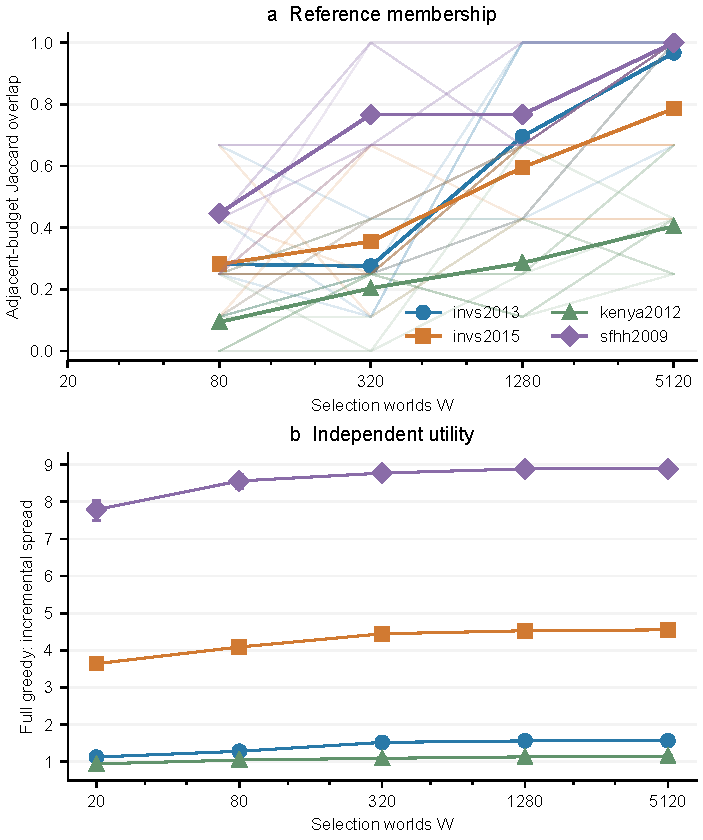
\includegraphics[width=\linewidth]{Fig1.pdf}
\caption{Reference membership and independent utility on four real networks ($k=5$, $p=0.01$, $h=3$, step coupling). (a) Thin lines show all ten path trajectories per network; thick lines show mean adjacent-budget Jaccard overlap. (b) Mean full-greedy incremental spread with 95\% percentile bootstrap intervals over ten paths. Evaluation uses 10,000 disjoint worlds per path. Intervals concern computational paths on fixed graphs; they are not population-network intervals. Colours and marker shapes identify networks}\label{fig:reference}
\end{figure}
\subsection{Candidate rankings and practical loss}
At $W=5120$, weighted-degree $4k$ pools had the following mean paired spread differences (candidate minus full): invs2013: -0.064, invs2015: -0.202, kenya2012: -0.005, sfhh2009: -0.610. Figure~\ref{fig:effects} reports all six candidate types and the across-path intervals, rather than selecting the best pool for each graph.

In contrast, topology-degree and PageRank $4k$ pools reproduced 39/40 and 40/40 ordered full references, respectively. These were genuine restrictions: their twenty eligible nodes represented 5.0--26.7\% of each graph. PageRank therefore had exactly zero paired differences at this setting; degree differed only on one Kenya path, with a slightly higher independently estimated spread. These observations do not establish a universal ranking advantage or future-path equivalence.


\begin{table}[t]
\caption{Mean candidate-minus-full spread changes with reference resolution. W4 and D4 denote weighted-degree and topology-degree $4k$ pools. Each entry averages ten paired path comparisons; signs of means are descriptive, not separate significance claims.}\label{tab:budget-effects}
\centering
\begin{tabular}{lrrrr}
\toprule
Network & W4: 20 & W4: 5120 & D4: 20 & D4: 5120 \\
\midrule
invs2013 & 0.128 & -0.064 & 0.215 & 0.000 \\
invs2015 & 0.364 & -0.202 & 0.539 & 0.000 \\
kenya2012 & 0.126 & -0.005 & 0.127 & 0.001 \\
sfhh2009 & 0.006 & -0.610 & 0.222 & 0.000 \\
\bottomrule
\end{tabular}
\end{table}
Weighted $4k$ had positive mean differences against the low-budget full reference on all four graphs, but negative means against the highest-budget reference (Table~\ref{tab:budget-effects}). The reference quality therefore changes the apparent utility conclusion, not only the trace-match count. Topology degree also gained relative to the low-budget reference, while largely reproducing it at high resolution. This pattern is consistent with a reduced candidate space limiting noisy low-budget choices, but the present contrasts do not isolate that causal mechanism.

In the 24-contrast primary sign-test family, 14 contrasts survived Holm correction at 0.05 (14 with negative and 0 with positive mean differences). The exact tests assess positive/negative balance after dropping zero path differences; they do not test mean equivalence. All unadjusted and adjusted values, zero counts and activated-node effect sizes are supplied in Online Resource 1.

At matched $4k$ coverage, the topology-degree and historical-weighted-degree results can be compared without changing candidate count. Their differences concern the simulator's use of distinct edges rather than event-frequency edge probabilities. Random-pool repetitions are averaged within path and do not triple the inferential sample size.

\begin{figure}[htbp]
\centering
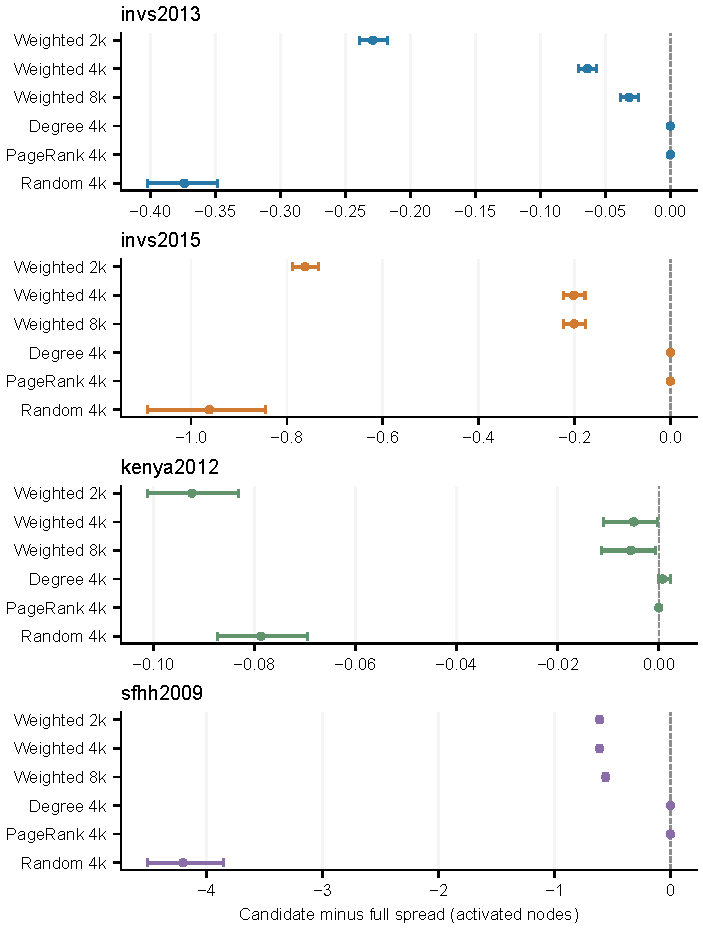
\includegraphics[width=\linewidth]{Fig2.pdf}
\caption{Primary candidate-minus-full spread differences at $W=5120$, $k=5$, $p=0.01$, $h=3$ under step coupling. Points are means of ten path-level differences; horizontal segments are 95\% percentile bootstrap intervals using 10,000 path resamples. Random $4k$ averages three pools within each path. All six candidate types are shown. Horizontal scales differ by network to retain small effects. Zero denotes the full reference, not an equivalence boundary}\label{fig:effects}
\end{figure}
\subsection{Time savings and loss tolerance}
For weighted $4k$ at the primary budget, mean selection-time savings were invs2013: 79.3\%, invs2015: 91.2\%, kenya2012: 74.9\%, sfhh2009: 95.2\%. These percentages exclude shared world preparation. The attributed full-pipeline savings, which include preparation and final evaluation, are reported separately in the source tables.

PageRank $4k$, which reproduced all forty primary references, saved 73.9--94.9\% of selection time across network means; after charging shared preparation and evaluation, savings were 58.0--83.8\%. These are observed cost advantages for this setting, not a guarantee at other budgets or on unseen graphs.

At a loss tolerance of 5\%, the point estimates met the threshold for 10/10 paths on invs2013, 7/10 paths on invs2015, 10/10 paths on kenya2012, 0/10 paths on sfhh2009. This is a description of point estimates at one chosen grid value, not evidence that 5\% is an acceptable application loss or a successful noninferiority test. Figure~\ref{fig:tradeoff} shows the entire prespecified tolerance grid.

\begin{figure}[htbp]
\centering
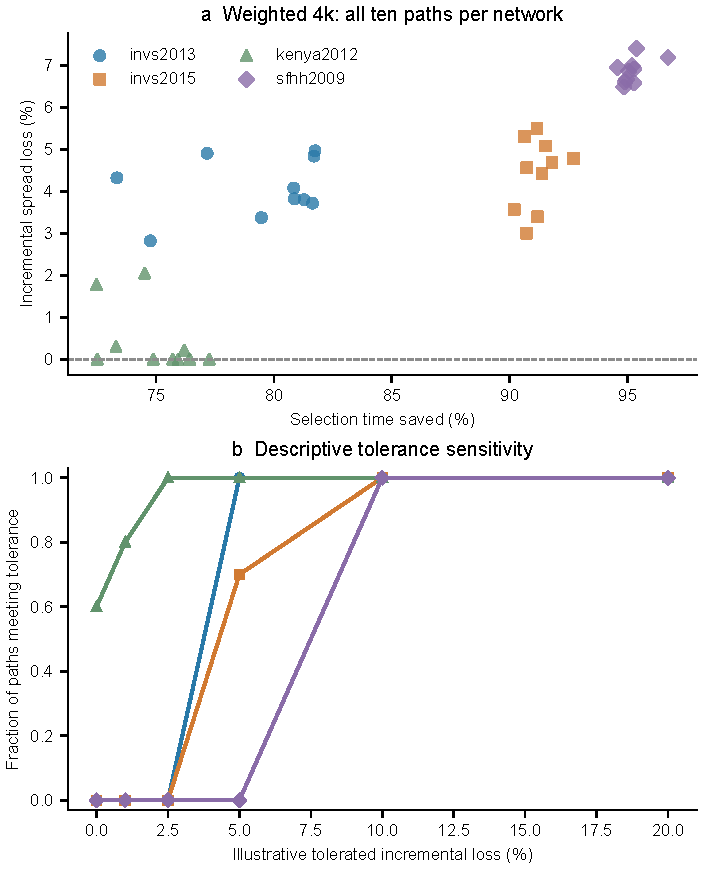
\includegraphics[width=\linewidth]{Fig3.pdf}
\caption{Cost and descriptive tolerance for the prespecified weighted $4k$ diagnostic at $W=5120$. (a) Every one of ten paths per real network is shown; the horizontal axis is selection-only time saving, and the vertical axis is loss relative to full incremental spread. Negative loss denotes a higher candidate estimate. (b) Fraction of paths whose point estimate meets each illustrative tolerance. These are fixed-grid descriptions with a point-estimate denominator, not inferential preservation decisions. All other candidate types remain in the source tables}\label{fig:tradeoff}
\end{figure}
\subsection{Propagation, coupling and structural sensitivity}
The predefined parameter and coupling controls extend the primary setting without changing the candidate rankings. Table~\ref{tab:sensitivity} gives the weighted $4k$ comparison at representative predefined conditions; Figure~\ref{fig:sensitivity} shows all five propagation settings, both couplings and both synthetic instances for its designated panels.

\begin{table}[t]
\caption{Mean weighted $4k$ minus full spread differences. First two columns vary transmission probability at $W=320,h=3$; last two compare couplings at $W=1280,p=0.01,h=3$. Ten paths per cell.}\label{tab:sensitivity}
\centering
\begin{tabular}{lrrrr}
\toprule
Network & $p=.005$ & $p=.05$ & Step & Fixed edge \\
\midrule
invs2013 & 0.004 & -0.513 & -0.065 & -0.061 \\
invs2015 & -0.019 & -1.526 & -0.205 & -0.206 \\
kenya2012 & 0.016 & 0.079 & 0.001 & 0.002 \\
sfhh2009 & -0.228 & -4.983 & -0.630 & -0.616 \\
\bottomrule
\end{tabular}
\end{table}
These contrasts identify sensitivity within the specified grid. They do not establish that one coupling estimates real diffusion more accurately. The two synthetic instances contain 2,000 nodes each, but have only one generated topology of each type. Their five paths measure computational variability on that topology; their agreement cannot substitute for additional real-network evidence. The $k=20$ results similarly retain saturated pools as controls and are tabulated separately.

\begin{figure}[htbp]
\centering
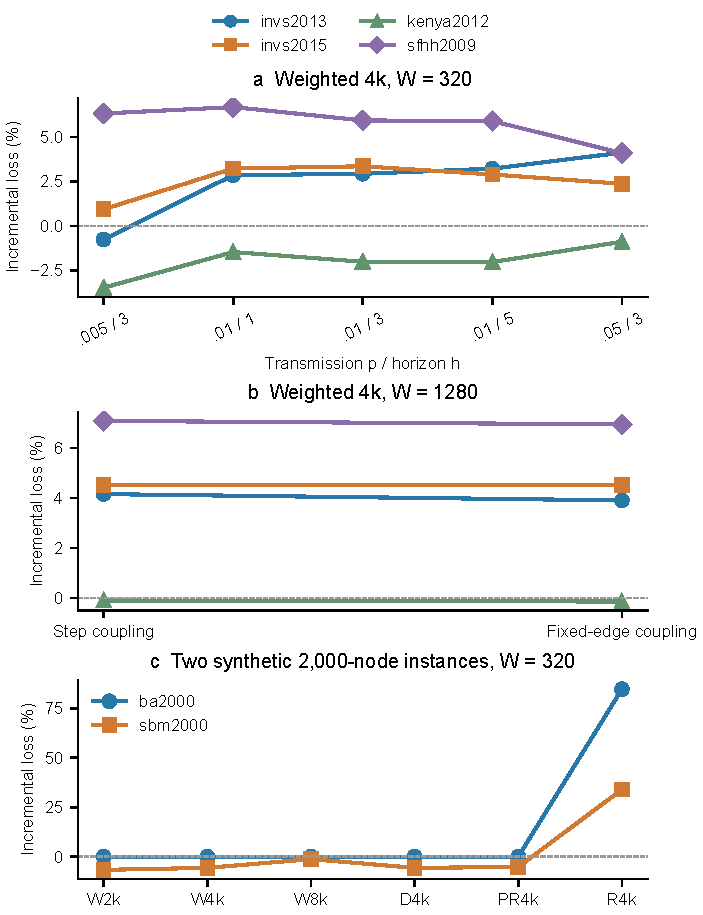
\includegraphics[width=\linewidth]{Fig4.pdf}
\caption{Predefined sensitivity panels. (a) Weighted $4k$ mean incremental loss across ten paths at $W=320$ for all five $(p,h)$ settings, including the primary setting. (b) The same candidate type under step and fixed-edge coupling at $W=1280$. (c) All six candidate types on two explicitly synthetic 2,000-node instances at $W=320$, five paths each; W/D/PR/R denote weighted degree, degree, PageRank and random. Lines connect tested settings without implying interpolation. These panels are descriptive means; all path values and uncertainty summaries are supplied as source data}\label{fig:sensitivity}
\end{figure}
\subsection{Repeated timing}
The five additional repetitions per real graph and arm produced 180 timing observations. Selected sets and all evaluated spreads were unchanged within those repetitions. Figure~\ref{fig:timing} separates selection and evaluation. Repetition measures execution variability in the compiled implementation; it does not increase the number of independent utility observations. Common world preparation and graph preparation remain outside the stacked bars and inside the separately reported full-pipeline attribution.

\begin{figure}[htbp]
\centering
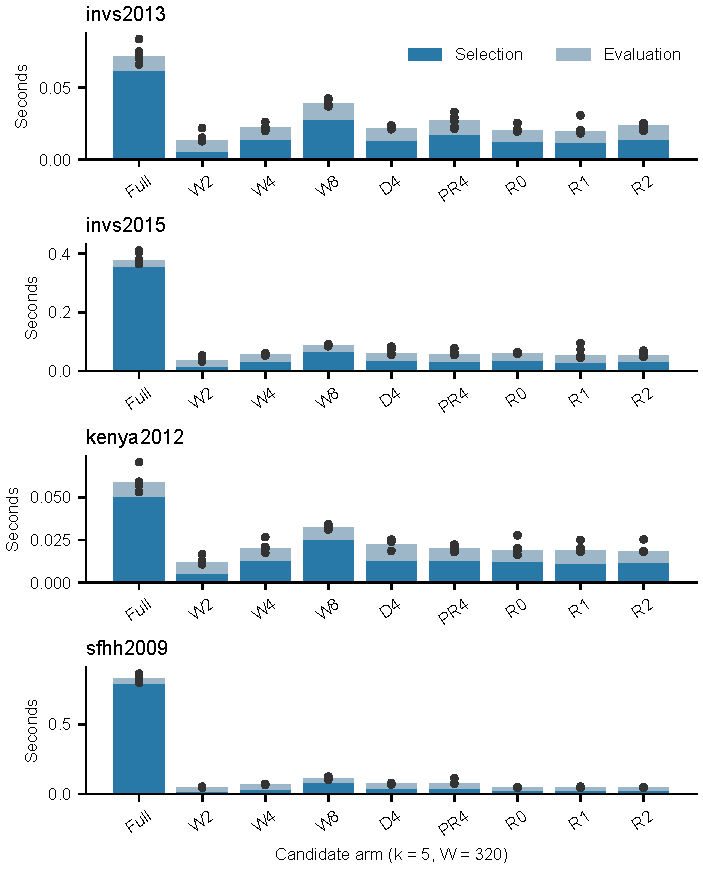
\includegraphics[width=\linewidth]{Fig5.pdf}
\caption{Repeated timing at $k=5,W=320$, path 1001, $p=0.01,h=3$, step coupling. Bars stack the median selection and evaluation times over five additional randomized serial repetitions; dots show each repetition's total of those phases. Full and all eight restricted executions are retained. W2/W4/W8 denote weighted pools; D4 and PR4 denote topology-degree and PageRank; R0--R2 are separate random pools. Shared preprocessing and JIT compilation are excluded from this figure and reported separately}\label{fig:timing}
\end{figure}
